\documentclass[]{aiaa-tc} % insert '[draft]' option to show overfull boxes

 \title{An application of Graph Theory to MDAO problem formulation}
        
\author{
  David Pate, %
     \thanks{Georgia Tech}
  Dr. Brian German 
     \thanks{Georgia Tech...}
  Justin Gray,%
     \thanks{Aerospace Engineer, MDAO Branch, Mail Stop 5-11, AIAA Member}   
 }
 
 



%\usepackage{setspace}
%\doublespace

\usepackage{graphicx}
\usepackage{wrapfig}
\usepackage{caption} 
\usepackage{amsmath}
\usepackage{lscape}
\usepackage{hyperref}
\usepackage{appendix}
\usepackage[section]{placeins}

\captionsetup[figure]{margin=5pt,font=small,labelfont=bf,textfont=bf,justification=justified,}
%\captionsetup[wrapfigure]{margin=5pt,font=small,labelfont=bf,justification=justified,singlelinecheck=off}
\captionsetup[table]{margin=5pt,font=small,labelfont=bf,textfont=bf,justification=justified,position=top}

\bibliographystyle{aiaa}

\usepackage{lettrine}
\usepackage{verbatim}

%\usepackage{hyperref} %allows for the creation of actual text links
\begin{document}

\maketitle
 
\begin{abstract}
   blah blah blah
\end{abstract}

\section*{Nomenclature}

\begin{tabular}{l l} 
    AAO      & All-At- \\
    MDAO     & Multidisciplinary Design Analysis and Optimization \\
    FPF      & Fundamental Problem Formulation \\
\end{tabular}


\section{Introduction}
    
    As the size and complexity of engineering systems grows the time and expense for setting up 
    analysis models grows with them. Multidisciplinary Design Analysis and Optimization (MDAO)
    frameworks such as OpenMDAO\cite{Gray2012} and ModelCenter have enabled a new level of analysis tool integration 
    and paved the way for models of with more analysis tools and increasing numbers of multidisciplinary couplings. 
    Such complex models present a distinct challenge proper implementation of any given solution strategy . 
    In fact as the size of a problem grows very large even determining what the proper solution strategy can be a daunting 
    task. 

    What is needed, in order to address the complexity problem, is a syntax for specifying an engineering problem 
    in a way that allows for both analysis of potential solution strategies and automated implementation of those strategies 
    inside an MDAO framework. In order to serve that purpose, the problem formulation needs to include the following information: 
    \begin{itemize}
       \item Discipline Analyses 
       \item Discipline State Variables and Residuals
       \item Local \& Global Design Variables
       \item Local \& Global Constraints
       \item Objective or Objectives
       \item Coupling Constraints
       \item Local and Global Parameters
    \end{itemize}
    Notably absent from the preceding list are any kind of solvers, optimizers, or other iterative solution finding tools. 
    At it most basic, a problem formulation includes only information about what is being sought after in a given problem, or what the
    goals of a given problem are. It need not contain any information about solution paths or strategies to reach those goals. 
    A general specification is one that states nothing specific about a problem solution path. 

    We define a complete and general problem specification striped down to it's most essential parts to be the 
    Fundamental Problem Formulation (FPF). By definition, the FPF for any given problem will be constant regardless 
    of which MDAO framework, optimization architecture, optimizer, or solver is used to solve the problem.

    In this work we proposed a graph based syntax for the specification of problem formulation. This graph based syntax provides several key
    features that make it useful for working with large scale MDAO problems. It provides a rigid structure that can be easily manipulated 
    with a wide range of well establish graph-theory algorithms for the purposes of problem decomposition. The graph syntax also 
    provides a means for algorithmically testing a given problem formulation to check if it is the FPF, and if not, to reduce it to the FPF. 
    Lastly, a graph based specification for problem formulation lends itself well to interacting with MDAO frameworks which dramatically 
    increases it's utility for real world applications. 


\section{Problem Formulation Syntax}
    The most common problem formulation syntax for an MDAO problem could be given as follows: 

    \begin{align}
        min &\ \ f\left(X\right) \notag
        \\ w.r.t. &\ \  X \notag
        \\ s.t. &\ \ G\left(X\right) \leq 0
        \\      &\ \ C\left(X\right) = 0
    \end{align}

    Where $f(X)$ is the objective function, $X$ is the vector of design variables, $G(X)$ are the optimization constraints, 
    and $C(X)$ are the coupling constraints. This does represent a general problem formulation, since it says nothing about 
    how the problem should be solved. Tedford and Martins used this format to specify the FPF for a set of test problems and 
    also to describe specific formulations for solving them with a number of optimization architectures\cite{Tedford2009}. Their
    work demonstrates clearly how multiple specific problem formulations can all relate back to a common FPF. 

    The challenge with using this traditional mathematical syntax is that it is not easily manipulated or analyzed by computer programs. 
    A number of matrix based methods have been used successfully to translate the mathematical syntax into a more useful computational form. 
    Steward's Design Structure Matrix (DSM) is a form of an adjacency matrix which captures the relationship between analysis tools where off 
    diagonal elements of the matrix indicate coupling\cite{Steward1981}. Figure \ref{fig:dsm_simple} shows a simple notional example of a DSM. 
    The DSM has been successfully applied in a number of ways to algorithmically modify problem formulations to 
    improve computational efficiency. Rogers et. al developed DeMAID to manipulate a
    DSM  minimizing the computational costs of solving highly coupled systems\cite{Rogers1996}. Lu and Martins demonstrated 
    the use of a weighted DSM to make partitioning and coordinating choices that dramatically reduced the 
    cost of solving a specific kind of optimization problem as the scale of the problem grew. 
    They applied weights to both the nodes (diagonal terms) and the edges (off diagonal terms) of the 
    DSM to indicated computational cost and coupling strength respectively.

    \begin{figure}[!hbp]
        \begin{center}
        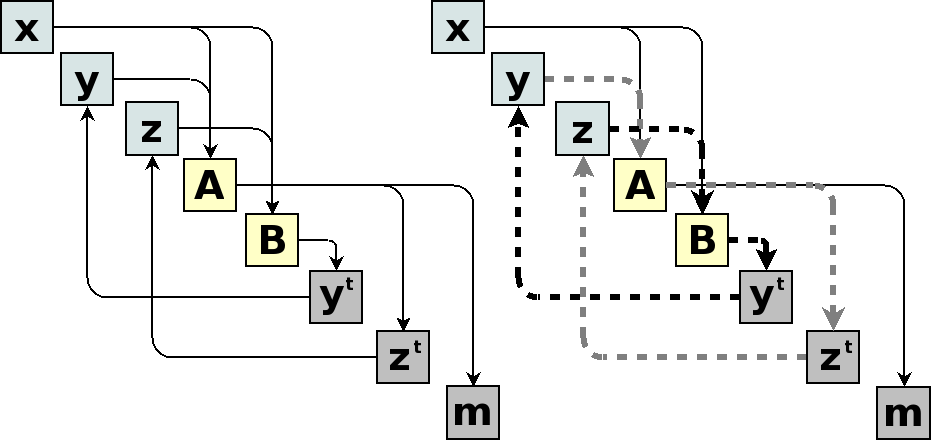
\includegraphics[width=.75\textwidth]{images/dsm_simple}
        \caption{Graph and matrix based DSM specifications for a notional analysis \label{fig:dsm_simple}}
        \end{center}
    \end{figure}

    Since a DSM describes a square adjacency matrix, it can be represented in an equivalent directed graph where nodes represent analysis tools and 
    edges represent information exchange between those tools. An alternate matrix based syntax, called a 
    Functional Dependence Table (FDT), was proposed by Michelena and Papalambros. 
    FDT represents the relationship between functions, including objectives and constraints, and their values\cite{Michelena1997}. Similar to DSM
    FDT also describes an adjacency matrix of a graph. Unlike the DSM graph, however, a FDT graph is an undirected 
    graph where nodes can represent analysis tools, objectives, or constraints. Edges between nodes represent a dependence on the same 
    variable value. By searching the FDT graph for clusters of totally connected nodes Wagner and Papalambros were identify groups of 
    analysis tools that were all dependent on the same input variables and used that to make partitioning decisions \cite{Wagner1993}. 

    It is possible to combine the syntax of an FDT and a DSM by making a subtle extension to a traditional DSM specification. Normally, a DSM is given 
    with analysis tools as nodes and variable dependencies given as edges. Lamb and Martins included the variables, objectives, and constraint functions
    as nodes in an Extented DSM (XDSM)\cite{Lambe2012} in order to capture a more complete problem formulation for MDAO problems. With XDSM 
    it is possible to also encompass the relationships defined in an FDT. Figure \ref{fig:dsm_full} 
    illustrates the same notional analysis as in Figure \ref{fig:dsm_simple} represented as an XDSM. 
    The dashed boxes indicate groups of nodes that could be collapsed back down to retrieve the simpler 
    DSM from above. Beyond specifying relationships between data in a problem formulation, XDSM also includes syntax to describe the
    procedural order of any given solution path. Figure \ref{fig:xdsm_full} shows the full XDSM specification for solving the notional 
    analysis with a traditional Multidisciplinary Design Feasible (MDF) architecture. 

    \begin{figure}[!hbp]
        \begin{center}
        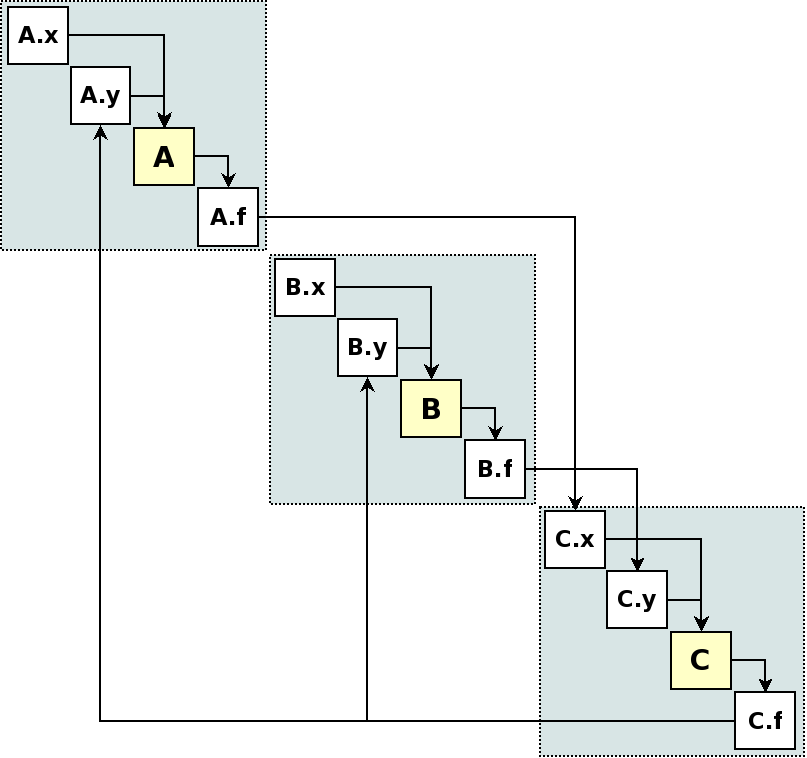
\includegraphics[width=.75\textwidth]{images/dsm_full}
        \caption{Extended DSM graph for a notional analysis \label{fig:dsm_full}}
        \end{center}
    \end{figure}

    
\section{Graph Based Problem Formulation Syntax}
    \subsection{Formulation Graph Syntax}
    Rather than start with an adjacency, we chose to work directly with a directed cyclic graph to develop a syntax for the FPF. 
    \begin{itemize}
        \item Specify analyses
        \item Connections between analyses 
            \begin{itemize}
                \item local variables
                \item global variables? Use "fake" node that broadcasts out to the rest of the graph? 
            \end{itemize}
        \item Cycles indicate coupling
        \item Cycles for design variables->objectives/constraints
        \item Objectives/constraints are just outputs? Special nodes? 
        \item Residuals are just outputs? Special nodes? 
        \item Parameters are just input nodes that are not design variables (use identifies these)
        \item FPF no solvers/optimizers anywhere in it
    \end{itemize}

    \subsection{Solution Graph Syntax}
    What is the difference between a problem formulation and a problem solution method? Convert from a cyclic graph, to an acyclic graph
    \begin{itemize}
        \item cycles indicate convergence loops or design varaible loops
        \item Problem can't be solved until all loops are *removed* by adding in solvers/optimizers
        \item *special* nodes for solvers and optimizers that *break* loops (from an algorithmic point of view)
        \item FPF represents the minimal amount of information necessary to define a problem
        \item Any solution path grows the graph complexity by adding edges and nodes (or possibly have an empty solution graph, which you build up 
        as you remove edges from problem formulation graph?)
    \end{itemize}

    
\section{Example Problem}

\section{Applications}

\section{Conclusions}

\bibliography{library}
\end{document}